% =====================================================================
%  第 2 章 辛几何与伪全纯曲线入门（后半）
%  ch02b —— 页段：PDF 63–90（原书 p.53–80），§2.5–§2.7 ＋ 第 2 章章末评注
% =====================================================================

% [原文 p.53]
这一点，正是近复结构几何与复几何不同、带有实几何性格的直接体现。其重要推论是下述事实。

设 $(M,J_M)$ 是凯勒流形。若存在从 $S^2$ 到 $M$ 的全纯映射，其同调类为 $\beta\in H_2(M;\Z)$，而该模空间的维数与虚拟维数都是 $0$，则即使把复结构 $J_M$ 动一动，仍然存在同调类为 $\beta$ 的、从 $S^2$ 出发的全纯映射。（准确地说，存在从 $S^2$ 的有限个并出发的全纯映射。）然而在近凯勒流形 $(M,J_M)$ 的情形，对某个“近复结构” $J_M$，即使存在同调类为 $\beta$ 的、从 $S^2$ 出发的伪全纯映射，一动 $J_M$ 它也可能消失。

这与下述情形类似。

对复曲面 $M$ 的两个复子流形 $N_1,N_2$，若作为集合的交 $N_1\cap N_2$ 非空，且 $N_1$ 与 $N_2$ 横截（transversal）相交，则 $[N_1]\cap[N_2]\in H_4(M)$（同调的帽积）不为 $0$。因此，即使把 $N_i$ 连续形变为 $N_i'$，$N_1'\cap N_2'$ 也非空。

而对一般的实子流形 $N_1,N_2$，同样的事情并不成立。

读到这里，诸位想必已经察觉到下面这一点了吧。

到此为止的论证中，辛结构究竟用在了哪里？仅仅从近复流形出发，又有什么不妥？实际上，像命题 2.38 那样的内容，对近复流形也能证明。因此，若到此为止的论证已经够用，那么用伪全纯曲线得到的便不是对辛几何的应用，而是对近复结构微分几何的应用。

辛结构真正派上用场的地方，是命题 2.39，即紧致性的证明。正因如此，紧致性的证明才是伪全纯曲线理论的中心。下面就另起一节吧。

\section{Morse 理论的观点与紧致性}

本节的目的，是在有限维类比所能说明的范围内，说明命题 2.39 的证明。理解“为什么证明伪全纯映射模空间的紧致性需要辛结构”，是本节的主要目的。

\takeaway{本节把伪全纯曲线看成环路空间 $\Omega_0(M)$ 上泛函 $A$ 的梯度流积分曲线（Floer 的观点），并用先验估计把“模空间紧致”归结为“能量有界时 $\|d\varphi\|$ 一致有界”；工具是 Weitzenböck 公式与 $A$ 的类梯度性。}

% [原文 p.54]
首先，说明把伪全纯曲线看作环路空间上梯度向量场的积分曲线这一 Floer 的立场。设 $(M,\omega_M)$ 是辛流形，$J_M$ 是与 $\omega_M$ 相容的 $M$ 的近复结构。如 §2.3 所述，$\omega_M,J_M$ 决定 $M$ 的 Hermite 度量 $g_M$。把从 $S^1$ 到 $M$ 的映射全体记作 $\Omega(M)$，称为 $M$ 的\textbf{环路空间}。把由与一点同伦的元素全体构成的、$\Omega(M)$ 的连通分支记作 $\Omega_0(M)$。本节并不做完备化去展开泛函分析，因此 $\Omega(M)$ 的拓扑暂时并不重要，先赋以 $C^\infty$ 拓扑即可。

按如下方式定义 $\Omega_0(M)$ 上的多值函数 $A$。取 $\ell\colon S^1\to M$，设 $\ell\in\Omega_0(M)$。于是存在 $u\colon D^2\to M$ 使 $u|_{S^1}=\ell$。

\begin{definition}{2.60}
\[
  A(\ell)=\int_{D^2}u^*\omega .
\]
\end{definition}

$A$ 是多值函数。先把这一点的含糊之处消除掉。为此取 $\Omega_0(M)$ 的覆盖空间（covering space）。考虑 $\ell\in\Omega_0(M)$、$u\colon D^2\to M$、$u|_{S^1}=\ell$ 这样的组 $(\ell,u)$ 的全体。所谓 $(\ell,u)\sim(\ell',u')$，是指 $\ell=\ell'$ 且 $u$ 与 $u'$ 作为 $\pi_2(M,\ell(S^1))$ 的元素一致。$\sim$ 显然是等价关系。把这个商空间记作 $\widetilde{\Omega}_0(M)$。$(\ell,u)\mapsto\ell$ 给出映射 $\widetilde{\Omega}_0(M)\to\Omega_0(M)$。容易看出 $\widetilde{\Omega}_0(M)$ 是 $\Omega_0(M)$ 的覆盖空间，其覆盖变换群（covering transformation group）是 $\pi_2(M)$。由 Stokes 定理，$A(\ell)$ 作为 $\widetilde{\Omega}_0(M)$ 上的函数是单值的。另一方面，设 $\gamma\in\pi_2(M)$，则
\begin{equation}
  A(\gamma\cdot(\ell,u))=A(\ell,u)+c(\gamma) \tag{2.21}
\end{equation}
成立。这里 $c(\gamma)=\int_{S^2}\gamma^*\omega$，由式 (2.21) 可知，$dA$ 是 $\Omega_0(M)$ 上的微分 $1$ 形式向 $\widetilde{\Omega}_0(M)$ 的拉回。为简单起见，仍把它写作 $dA$。显然 $dA$ 是闭微分形式。（由于 $A$ 不是单值的，$dA$ 未必是恰当形式（exact $1$ form）。）

% [Tutor Note: $A$ 只有在覆盖空间 $\widetilde{\Omega}_0(M)$ 上才是单值函数；式 (2.21) 表明 $A$ 沿 $\pi_2(M)$ 的平移改变一个常数 $c(\gamma)$，这正是后来 Floer 同调取 Novikov 环系数的根源。]

% [原文 p.55]
用 $M$ 上的黎曼度量 $g_M$，把 $\Omega_0(M)$ 上的黎曼度量 $\tilde g$ 定义为
\[
  \tilde g(X,Y)=\int g_M(X(t),Y(t))\,dt .
\]
这里 $X,Y\in T_\ell(\Omega_0(M))=\Gamma(S^1;\ell^*TM)$。由 $\tilde g$ 与 $dA$，$\Omega_0(M)$ 上的向量场 $\operatorname{grad}A$ 由下式确定：
\begin{equation}
  \tilde g(\operatorname{grad}A,V)=dA(V). \tag{2.22}
\end{equation}

\begin{remark}{2.61}
  系统地研究了由闭微分形式经 (2.22) 确定的向量场的 Morse 理论（在有限维情形）的是 Novikov [287]。§5.2 将说明 Novikov 的理论。
\end{remark}

\begin{proposition*}{2.62}
  对 $\ell\in\Omega_0(M)$，
  \begin{equation}
    \operatorname{grad}_\ell A+J_M\left(\frac{d\ell}{dt}\right)=0 \tag{2.23}
  \end{equation}
  成立。这里左边是 $\Gamma(S^1;\ell^*TM)=T_\ell(\Omega(M))$ 的元素。
\end{proposition*}

\begin{proof}
  取 $\gamma\colon(-\varepsilon,\varepsilon)\to\Omega(M)$ 为满足 $\gamma(0)=\ell$ 的光滑道路。固定一个满足 $u|_{S^1}=\ell$ 的 $u$。$\gamma$ 给出映射 $(-\varepsilon,\varepsilon)\times S^1\to M$，把它写作 $\tilde\gamma$。把 $\tilde\gamma$ 在 $[0,\tau]\times S^1$ 上的限制与 $u$ 按图 2.2 粘合所得的映射记作 $u_\tau$。此时 $u_\tau|_{S^1}=\gamma(\tau)$。因此
  \begin{equation}
    A(\gamma(\tau))=\int_{D^2}u_\tau^*\omega . \tag{2.24}
  \end{equation}

  \begin{figure}[htbp]
    \centering
    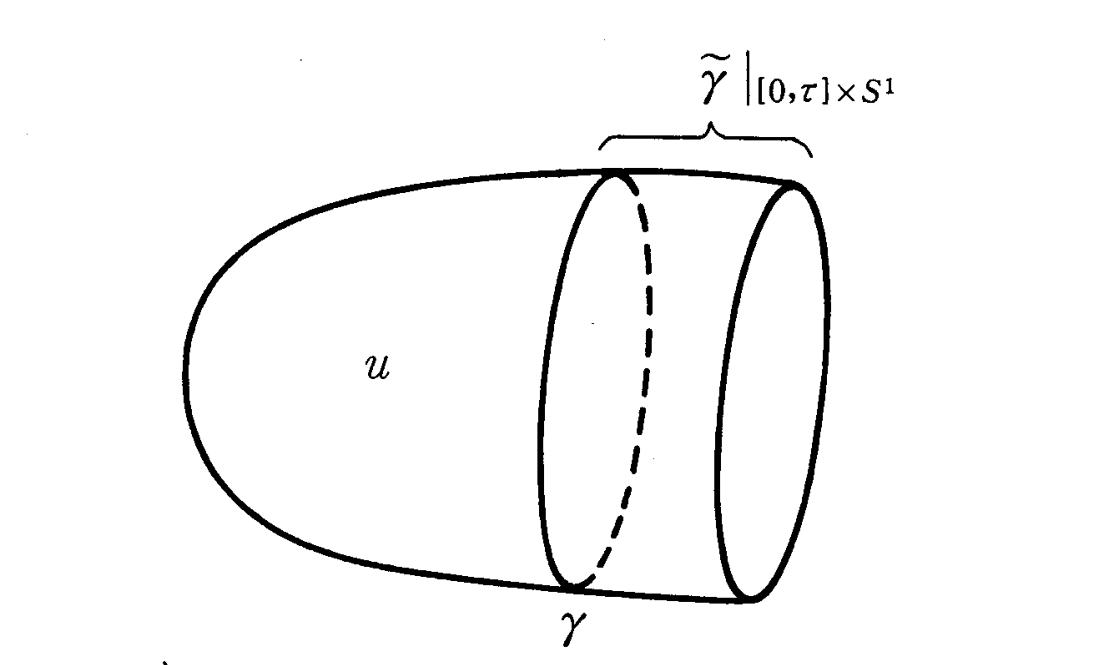
\includegraphics[width=0.55\textwidth]{figures/fig2.2.png}
    \figtitle{2.2}{$\tilde\gamma$ 在 $[0,\tau]\times S^1$ 上的限制与 $u$ 的粘合（原书 p.55）}
  \end{figure}

% [Tutor Note: 式 (2.22) 里的 $\operatorname{grad}$ 是在环路空间的 $L^2$ 度量 $\tilde g$ 下取的，而不是 $M$ 上的梯度；$\tilde g$ 由 Hermite 度量 $g_M$ 沿环路积分得到，故 $T_\ell\Omega$ 中的向量要先逐点配对再积分。]

% [原文 p.56]
令 $X=\left.\dfrac{d\gamma}{d\tau}\right|_{\tau=0}\in T_\ell(\Omega_0(M))=\Gamma(S^1;\ell^*TM)$。由 (2.24) 得
\begin{equation}
  \frac{\partial A(\gamma(\tau))}{\partial\tau}
  =\int_{t\in S^1}\omega\left(X(\ell(t)),\frac{d\ell}{dt}\right)dt \tag{2.25}
\end{equation}
成立。由 (2.22)，(2.25) 的左边是 $\tilde g(\operatorname{grad}A,X)$。于是
\[
  -\int_{t\in S^1}\omega\left(\frac{d\ell}{dt},X(\ell(t))\right)dt
  =\int_{t\in S^1}g_M(\operatorname{grad}A,X(\ell(t)))\,dt .
\]
这正是 (2.23) 的意思。
\end{proof}

把命题 2.62 换一种说法，$A$ 与伪全纯曲线的关系就清楚了。与引理的证明中一样，考虑 $\gamma\colon(-\varepsilon,\varepsilon)\to\Omega(M)$ 与 $\tilde\gamma\colon(-\varepsilon,\varepsilon)\times S^1\to M$。

\begin{corollary*}{2.63}
  $\gamma\colon(-\varepsilon,\varepsilon)\to\Omega(M)$ 是 $\operatorname{grad}A$ 的积分曲线，与 $\tilde\gamma\colon(-\varepsilon,\varepsilon)\times S^1\to M$ 是伪全纯映射，二者等价。
\end{corollary*}

由命题 2.62 与 $J(\partial/\partial t)=-\partial/\partial\tau$ 即知此结论。

为使后面的话更易读，把与辛结构相容的近复结构这一概念、以及梯度向量场这一概念稍作推广。

\begin{definition}{2.64}
  近复结构 $J_M$ 关于 $\omega_M$ \textbf{温和}（$J_M$ is tamed by $\omega_M$），是指对任意非零切向量 $V$，都有 $\omega_M(V,J_MV)>0$。
\end{definition}

当 $J_M$ 关于 $\omega_M$ 温和时，用
\[
  2g_M(V,W)=\omega_M(V,J_MW)+\omega_M(W,J_MV)
\]
定义黎曼度量 $g_M$。再用 $g_M$ 同样地确定 $\Omega(M)$ 上的度量 $\tilde g$。

\begin{definition}{2.65}
  设流形上有向量场 $X$ 与函数 $f$。称 $X$ 关于 $f$ 是\textbf{类梯度的}（gradient like），是指存在正数 $c$ 使 $X(f)\ge c\|X\|^2$ 成立。即使 $f$ 是本节所考虑的多值函数 $A$，这个术语也仍然有意义。
\end{definition}

\begin{remark}{2.66}
  在力学系统的术语中，$f$ 称为 $X$ 的 Lyapunov 函数（Lyapunov function）。
\end{remark}

% [Tutor Note: 定义 2.64 的“温和”比“相容”弱：相容还要求 $\omega_M(J_MV,J_MW)=\omega_M(V,W)$（即 $J_M$ 保持 $\omega_M$），温和只要求 $\omega_M(V,J_MV)>0$。所以下面用两项对称化定义 $g_M$，此时 $g_M$ 只是黎曼度量，未必与 $J_M$ 相容。]

$f$ 的梯度向量场关于 $f$ 是类梯度的。实际上

% [原文 p.57]
\[
  \operatorname{grad}f(f)=df(\operatorname{grad}f)=g_M(\operatorname{grad}f,\operatorname{grad}f)=\|\operatorname{grad}f\|^2 .
\]

如今用这些术语，命题 2.62 便可作如下推广。设 $J_M$ 是关于 $\omega_M$ 温和的近复结构。$J_M\left(\dfrac{d\ell}{dt}\right)$ 是 $\Omega(M)$ 上的向量场。

\begin{lemma*}{2.67}
  $-J_M\left(\dfrac{d\ell}{dt}\right)$ 关于 $A$ 是类梯度的。
\end{lemma*}

\begin{proof}
  沿着命题 2.62 的证明中的计算走一遍，得
  \[
    -J_M\left(\frac{d\ell}{dt}\right)_\ell(A)
    =\int\omega_M\left(\frac{d\ell}{dt},J_M\frac{d\ell}{dt}\right)dt .
  \]
  由定义，右边是 $\tilde g(d\ell/dt,d\ell/dt)$。
\end{proof}

下面叙述“类梯度”这一性质的重要推论。先考虑关于单值函数 $f$ 类梯度的向量场 $X$。设 $\gamma\colon[a,b]\to M$ 是 $X$ 的积分曲线。

\begin{lemma*}{2.68}
  \[
    \int_a^b\left\|\frac{d\gamma}{d\tau}\right\|^2 d\tau\le C\,(f(b)-f(a)).
  \]
\end{lemma*}

\begin{proof}
  把 $\operatorname{grad}f\left(\dfrac{d\gamma}{d\tau}\right)\ge c\left\|\dfrac{d\gamma}{d\tau}\right\|^2$ 积分即可。
\end{proof}

% [Tutor Note: 命题 2.62 与引理 2.67 的符号不要弄混：沿 $-\operatorname{grad}A$ 的流（即 $\operatorname{grad}A$ 的反向）才是伪全纯曲线对应的方向；引理 2.67 说的是 $-J_M(d\ell/dt)$ 关于 $A$ 类梯度，故 $A$ 沿流的正向增加。]

想在 $f=A$ 这一无限维情形下使用引理 2.68。为此要定义映射的能量与体积，并说明伪全纯映射、调和映射、极小子曲面之间的关系。设 $\varphi\colon N\to M$ 是黎曼流形之间的光滑映射，用局部坐标写作 $\varphi=(\varphi_1,\dots,\varphi_m)$。设 $g_{N,ij},g_{M,ij}$ 是用局部坐标写出的黎曼度量，各自的逆矩阵记作 $g_N^{ij},g_M^{ij}$。

\begin{definition}{2.69}
  \[
    \mathcal{E}(\varphi)=\frac12\int_N\sum_{i,j,k,\ell}g_N^{k\ell}g_{M,ij}
    \frac{\partial\varphi_i}{\partial x_k}\frac{\partial\varphi_j}{\partial x_\ell}
    \sqrt{\det(g_{N,ab})}\,dx_1\cdots dx_n
  \]
  并称 $\mathcal{E}(\varphi)$ 为 $\varphi$ 的\textbf{能量}（energy）。
\end{definition}

% [原文 p.58]
\begin{definition}{2.70}
  \[
    \operatorname{Vol}(\varphi)=\int_N\sqrt{\det\left(\sum_{i,j}g_{M,ij}
    \frac{\partial\varphi_i}{\partial x_k}\frac{\partial\varphi_j}{\partial x_\ell}\right)}
    \,dx_1\cdots dx_n
  \]
  并称 $\operatorname{Vol}(\varphi)$ 为 $\varphi$ 的\textbf{体积}（volume）（括号中的矩阵是以 $k,\ell$ 为下标的 $n\times n$ 矩阵）。要注意，体积不依赖于 $N$ 的度量。
\end{definition}

% [Tutor Note: 定义 2.70 中被积式的行列式与 $N$ 的度量无关：作坐标变换时 $(\partial\varphi/\partial x)$ 按 Jacobi 矩阵变换，其行列式平方与 $dx_1\cdots dx_n$ 的变换因子恰好相消。故 $\operatorname{Vol}(\varphi)$ 只依赖 $g_M$ 与 $\varphi$ 的像。]

把上面的定义稍作改写。取 $e_1,\dots,e_n\in T_pN$ 为 $T_pN$ 关于 $g_{N,k\ell}$ 的正交规范基。用 $h_{k\ell}=g_M(d\varphi(e_k),d\varphi(e_\ell))$ 定义矩阵 $h_{k\ell}$。它的迹与行列式由
\[
  \operatorname{Tr}(d\varphi)=\sum_{k=1}^n h_{kk},\qquad
  \operatorname{Det}(d\varphi)=\det(h_{k\ell})
\]
定义。$\operatorname{Tr}(d\varphi),\operatorname{Det}(d\varphi)$ 不依赖于正交规范基的取法。设 $\Omega_N$ 为 $N$ 的体积元 $(\sqrt{\det(g_{N,ij})}\,dx_1\cdots dx_n)$。

\begin{lemma}{2.71}
  \[
    \mathcal{E}(\varphi)=\frac12\int_N\operatorname{Tr}(d\varphi)\,\Omega_N,
    \qquad
    \operatorname{Vol}(\varphi)=\int_N\operatorname{Det}(d\varphi)^{1/2}\,\Omega_N .
  \]
\end{lemma}

其证明容易，留给读者。

把使能量取极值的映射称为\textbf{调和映射}（harmonic map），把使体积取极值的浸入称为\textbf{极小浸入}（minimal immersion）。本书只用 $N$ 为 $2$ 维的情形，故以下设 $N$ 是 $2$ 维，并写作 $\Sigma$。$2$ 维这一情形的重要推论是下面的命题 2.73。先准备一个词。

\begin{definition}{2.72}
  称 $\varphi\colon\Sigma\to M$ 是\textbf{共形的}（conformal），是指存在函数 $h\colon\Sigma\to\R_+$，使
  \[
    g_M(d\varphi(V),d\varphi(W))=h(p)\,g_\Sigma(V,W)
  \]
  对任意 $V,W\in T_p\Sigma$ 成立。共形的微分同胚称为\textbf{共形变换}（conformal transformation）。
\end{definition}

\begin{proposition*}{2.73}
  $2$ 维流形 $\Sigma$ 出发的映射的能量，在 $\Sigma$ 的共形变换下不变。即：若 $\phi\colon\Sigma\to\Sigma$ 是共形变换、$\varphi\colon\Sigma\to M$ 是任意映射，则 $\mathcal{E}(\varphi)=\mathcal{E}(\varphi\circ\phi)$。
\end{proposition*}

\begin{proof}
  设 $g_M(d\phi(V),d\phi(W))=h(p)g_\Sigma(V,W)$，则由定义容易得到

% [原文 p.59]
$e_{\varphi\circ\phi}(p)=h(p)^2e_\varphi(\phi(p))$。对面积元有 $\phi^*\Omega_\Sigma(p)=h(p)^{-2}\Omega_\Sigma(p)$ 成立。由这两式与引理 2.71 即得命题 2.73。
\end{proof}

极小浸入与调和映射的关系由下面的命题 2.74 与命题 2.76 给出。此后一段时间内，为了对能量标明 $\Sigma$ 的度量，写作 $\mathcal{E}(\varphi;g_\Sigma)$。

\begin{proposition*}{2.74}
  映射 $\varphi\colon(\Sigma,g_\Sigma)\to(M,g_M)$ 是共形的，等价于：对固定 $\varphi$ 而变动 $g_\Sigma$ 的变分，$\mathcal{E}(\varphi;g_\Sigma)$ 取最小值。
\end{proposition*}

\begin{proof}
  注意由算术平均与几何平均的关系得到的下述引理。
\end{proof}

\begin{lemma}{2.75}
  \[
    \frac{\operatorname{Tr}(d\varphi)(p)}{2}\ge\left(\operatorname{Det}(d\varphi)(p)\right)^{1/2}
  \]
  且等号成立当且仅当 $g_M(d\varphi(V),d\varphi(W))=c\,g_\Sigma(V,W)$ 对任意 $V,W\in T_p\Sigma$ 成立。
\end{lemma}

\begin{proof}[命题 2.74 的证明（续）]
  由引理 2.75 与体积不依赖 $N$ 的度量，得 $\mathcal{E}(\varphi;g_\Sigma)\ge\operatorname{Vol}(\varphi)$；等号成立当且仅当 $\varphi\colon(\Sigma,g_\Sigma)\to(M,g_M)$ 是共形的。由此即得命题 2.74。
\end{proof}

\begin{proposition*}{2.76}
  对共形的浸入 $\varphi$，是极小浸入与是调和映射二者等价。
\end{proposition*}

\begin{proof}
  令 $f(s,t)=\mathcal{E}(\varphi_s;\varphi_t^*g_\Sigma)$，则由 $\operatorname{Vol}(\varphi_\varepsilon)=\mathcal{E}(\varphi_\varepsilon;\varphi_\varepsilon^*g_\Sigma)$ 得 $\operatorname{Vol}(\varphi_\varepsilon)=f(\varepsilon,\varepsilon)$。另一方面由定义，$\mathcal{E}(\varphi_\varepsilon;g_\Sigma)=f(\varepsilon,0)$。又由命题 2.74，$\partial f/\partial t(0,0)=0$。由此
  \[
    \frac{d}{d\varepsilon}\operatorname{Vol}(\varphi_\varepsilon)(0)
    =\frac{d}{d\varepsilon}\mathcal{E}(\varphi_\varepsilon;g_\Sigma)(0).
  \]
  故命题 2.76 成立。
\end{proof}

% [Tutor Note: 命题 2.74 说的是“固定 $\varphi$、只动定义域度量 $g_\Sigma$”这一变分下的最小性，不是通常的映射变分；引理 2.75 正是两个平均值的比较，等号条件写成 $g_M(d\varphi(\cdot),d\varphi(\cdot))=c\,g_\Sigma$，即共形性。]

下面叙述与伪全纯映射的关系。设 $(M,g_M,\omega_M,J_M)$ 是近凯勒流形。（即假定 $J_M$ 与 $\omega_M$ 相容。）

\begin{lemma*}{2.77}
  对 $\varphi\colon\Sigma_M\to M$，
  \[
    \int_\Sigma\varphi^*\omega_M\le\operatorname{Vol}(\varphi).
  \]
\end{lemma*}

% [原文 p.60]
\begin{proof}
  取 $p\in\Sigma$，设 $(\tau,t)$ 是 $p$ 附近的 $\Sigma$ 的局部坐标。
  \begin{equation}
  \begin{aligned}
    \varphi^*\omega\left(\frac{\partial}{\partial\tau},\frac{\partial}{\partial t}\right)
    &=g_M\left(d\varphi\left(\frac{\partial}{\partial\tau}\right),
      J_Md\varphi\left(\frac{\partial}{\partial t}\right)\right)\\
    &\le\left\|d\varphi\left(\frac{\partial}{\partial\tau}\right)\right\|^{1/2}
      \left\|d\varphi\left(\frac{\partial}{\partial t}\right)\right\|^{1/2}.
  \end{aligned}
  \tag{2.26}
  \end{equation}
  左边积分得 $\int_\Sigma\varphi^*\omega_M$，右边积分得 $\operatorname{Vol}(\varphi)$。
\end{proof}

% [Tutor Note: 原书 p.60 的式 (2.26) 把右边两个范数的指数印作 $1/2$；按 Schwarz 不等式应为一次方，否则积分后得不到 $\operatorname{Vol}(\varphi)$。此处照抄原书，读者按 $\|a\|\,\|b\|$ 理解。]

\begin{lemma*}{2.78}
  若 $\varphi\colon\Sigma_M\to M$ 是伪全纯映射，则
  \[
    \int_\Sigma\varphi^*\omega_M=\operatorname{Vol}(\varphi).
  \]
\end{lemma*}

\begin{proof}
  在 $\Sigma$ 上取一点，使坐标在该点满足 $J_\Sigma(\partial/\partial\tau)=\partial/\partial t$，则 (2.26) 中等号成立。
\end{proof}

\begin{remark}{2.79}
  命题 2.76 与引理 2.77 对复维数 $2$ 以上的复子流形也同样成立（用 $\omega^n$ 代替 $\omega$）。这称为 Wirtinger 不等式（Wirtinger inequality）（见 [156] p.31）。
\end{remark}

\begin{remark}{2.80}
  引理 2.77 的左边只依赖 $\varphi(\Sigma)$ 的同调类。像这样用拓扑量从下方估计能量之类量的式子，称为 Bogomol'nyi 不等式（Bogomol'nyi inequality）（见 [398] 等）。其等号成立的情形称为 BPS 瞬子（Bogomol'nyi–Prasad–Sommerfeld instanton）。除刚出现的伪全纯曲线（或复子流形）以外，自对偶联络等也是其例（另见注 2.84）。
\end{remark}

由引理 2.77 与 2.78，利用 $\int_\Sigma\varphi^*\omega_M$ 在连续形变下不变，可知下述事实。

\begin{proposition}{2.81}
  伪全纯映射是极小映射。
\end{proposition}

进而，

\begin{proposition*}{2.82}
  伪全纯映射是共形映射。
\end{proposition*}

\begin{proof}
  对伪全纯映射 $\varphi\colon\Sigma\to M$，取 $V\in T_p\Sigma$，则由定义
  \[
    g_M(d\varphi(V),d\varphi(V))=g_M(J_Md\varphi(V),J_Md\varphi(V))
    =g_M(d\varphi(J_\Sigma V),d\varphi(J_\Sigma V)).
  \]
  $V,J_\Sigma V$ 是 $T_p\Sigma$ 的基，故 $\varphi$ 是共形的。
\end{proof}

% [原文 p.61]
\begin{corollary}{2.83}
  伪全纯映射是调和映射。
\end{corollary}

证明由命题 2.81, 2.82 显然。（当 $\varphi$ 不是浸入时，只需确认在 $\varphi$ 是浸入的点处满足调和映射的方程。这只要在该点的邻域内取非零变分，由命题 2.81, 2.82 即可推出。）

把“映射是调和映射”这一条件写成方程，就得到二阶非线性偏微分方程。另一方面，“映射是伪全纯映射”则由一阶非线性偏微分方程表达。系 2.83 等于把二阶微分方程的问题替换成了一阶微分方程的问题。

微分方程是一阶的，这一点在考虑模空间时很重要。也就是说，像前一节那样把微分方程看作无限维流形上无限维向量丛的截面时，要使线性化方程构成 Fredholm 算子，一阶方程更为方便。

把二阶微分方程的问题换成一阶微分方程，这一过程在别处也出现。（例如 Yang–Mills 方程与自对偶方程的关系就是如此。）这被认为与粒子物理中近来重要性日增的超对称性（super symmetry）有关。

\begin{remark}{2.84}
  黎曼流形 $M$ 上的闭微分 $k$ 形式 $\Omega$ 称为\textbf{校准}（calibration），是指对 $V_i\in T_pM$ 有 $|\Omega(V_1,\dots,V_k)|\le\|V_1\|\cdots\|V_k\|$ 成立。（此时 $\int_N\Omega\le\operatorname{Vol}N$ 成立。）

  对校准 $\Omega$，称 $k$ 维子流形 $N$ 为\textbf{被校准子流形}（calibrated submanifold），是指
  \[
    \Omega|_N=\omega_{g_M|N}
  \]
  成立。这里 $\Omega|_N$ 是 $\Omega$ 在 $N$ 上的限制，$\omega_{g_M|N}$ 是由 $M$ 的度量的限制所得的 $N$ 的黎曼度量的体积元。

  此条件与 $\int_N\Omega=\operatorname{Vol}N$ 等价。

  $\int_N\Omega$ 只依赖 $N$ 的同调类。另一方面 $\int_N\Omega\le\operatorname{Vol}N$ 总是成立。因此，被校准的子流形是极小子流形。

  在我们的情形，辛形式 $\omega$ 是校准。校准由 Harvey–Lawson [174] 为研究极小曲面而引入，近来在场论与弦理论中也受到关注（见 §6.6）。
\end{remark}

% [原文 p.62]
先回到“把引理 2.68 套用到我们的泛函 $A$ 上”这一目的。对 $\gamma\colon[a,b]\to\Omega(M)$，写作 $\tilde\gamma\colon[a,b]\times S^1\to M$。

\begin{lemma*}{2.85}
  若 $\tilde\gamma\colon[a,b]\times S^1\to M$ 是伪全纯映射，则
  \[
    \int_{[a,b]\times S^1}\left(\left\|\frac{\partial\tilde\gamma}{\partial t}\right\|^2
    +\left\|\frac{\partial\tilde\gamma}{\partial\tau}\right\|^2\right)d\tau dt
    \le C\int_{[a,b]\times S^1}\tilde\gamma^*\omega
  \]
  成立（$\tau$ 是 $[a,b]$ 的参数，$t$ 是 $S^1$ 的参数）。
\end{lemma*}

\begin{proof}
  若 $J_M$ 与 $\omega_M$ 相容，这就是引理 2.78。即使 $J_M$ 只满足比相容更弱的 $\omega_M$ 温和这一条件，把引理 2.67 与引理 2.68 的证明合起来也能证明。留给读者。
\end{proof}

\begin{remark}{2.86}
  引理 2.77 在 $J_M$ 关于 $\omega_M$ 仅为温和的情形也可如下推广。

  设 $\varphi\colon S^2\to M$ 是关于近复结构 $J_M'$ 的伪全纯曲线，且 $J_M'$ 关于 $\omega_M$ 温和。此时 $\mathcal{E}(\varphi)\le\varphi_*([S^2])\cap[\omega]$。

  证明只需利用 $S^2$ 去掉两点后与 $\R\times S^1$ 共形，把问题化归到引理 2.85 即可。
\end{remark}

% [Tutor Note: 注 2.86 里的近复结构记作 $J_M'$（带撇），与前面的 $J_M$ 不是同一个；此处只需 $J_M'$ 关于 $\omega_M$ 温和，不需要它可积或与 $\omega_M$ 相容。]

下面说明引理 2.68, 2.78, 2.85 与注 2.86，同模空间紧致性的关系。先设 $V$ 是有限维紧流形 $X$ 上关于单值函数 $f$ 类梯度的向量场。设 $\gamma\colon\R\to X$ 是 $V$ 的积分曲线。则引理 2.68 意味着
\begin{equation}
  \int_\R\left\|\frac{\partial\gamma}{\partial\tau}\right\|^2d\tau\le C(\sup f-\inf f) \tag{2.27}
\end{equation}
即 $\gamma$ 的一阶导数的 $L^2$ 范数一致有界。

一般地，给出一列偏微分方程的解 $\gamma_i$、想从中找出收敛子列时，有效的方法是下面这一套。

% [原文 p.63]
\textbf{处方 2.87}
\begin{enumerate}[label=（\arabic*）,leftmargin=2.8em]
  \item 首先，就某个较弱的范数证明 $\gamma_i$ 一致有界。
  \item 用微分方程本身，证明弱范数下的估计可以推出强范数下的估计。（例如用 $L^2$ 范数估计 Sobolev 范数。）若方程是椭圆型的，这常可与方程解的光滑性（regularity）的证明并行完成。
  \item 用 Rellich 定理，从关于强范数一致有界的函数列中找出关于弱范数收敛的子列。
  \item 再用 (2) 的方法，证明关于弱范数收敛的列其实关于强范数也收敛。
\end{enumerate}
\hfill$\square$

% [Tutor Note: 原书把这一条称为“处方 2.87”，它不是定理而是椭圆正则性论证的标准四步；其中 (1) 由引理 2.68, 2.78, 2.85、注 2.86 提供，(3) 的 Rellich 定理即 Sobolev 紧嵌入定理。]

要执行这套处方，首先需要 (1)，即关于某个弱范数的有界性。引理 2.68, 2.78, 2.85、注 2.86 提供的正是它。一旦向量场不再是类梯度的，或者近复结构不再关于 $\omega_M$ 温和，这些引理便不成立，紧致性随之崩溃。在本节末尾，就用引理 2.68 的情形看一个实例。

设 $X=S^2=\{(x,y,z)\mid x^2+y^2+z^2=1\}$，令 $f(x,y,z)=z$。$f$ 的梯度向量场 $V_0$ 如图 2.3 所示。

\begin{figure}[htbp]
  \centering
  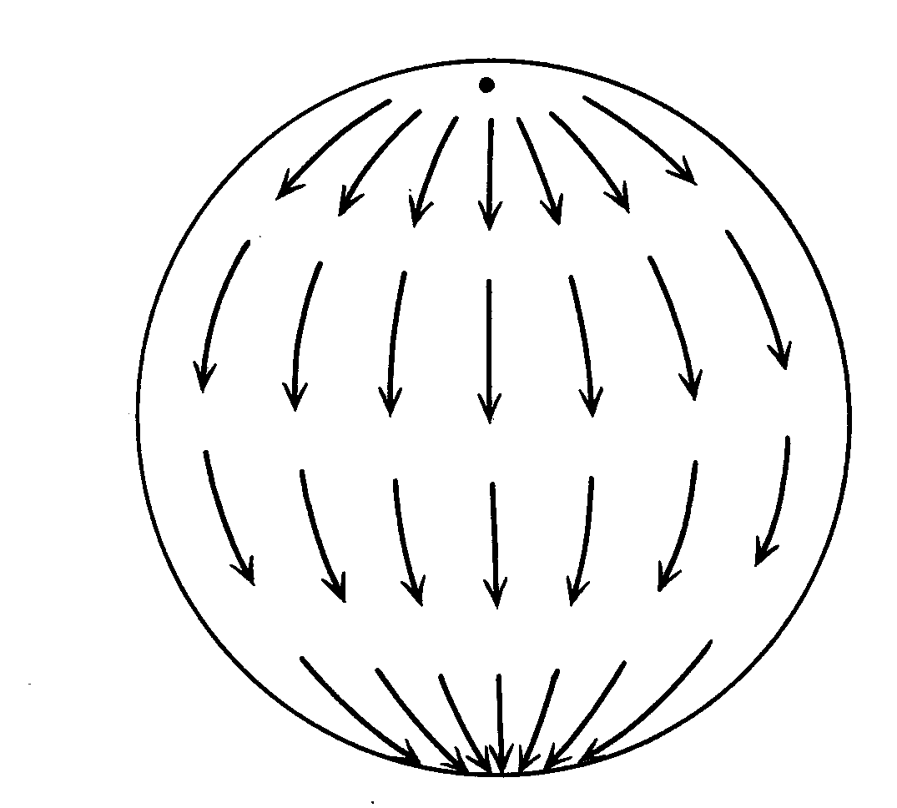
\includegraphics[width=0.34\textwidth]{figures/fig2.3.png}
  \figtitle{2.3}{$V_0=\operatorname{grad}f$（原书 p.63）}
\end{figure}

取 $W(x,y,z)=y\,\partial/\partial x-x\,\partial/\partial y$，定义 $X_\theta=(1-\chi(z)\theta)V+\chi(z)\theta W$（图 2.4）。这里 $\chi\colon[-1,1]\to[0,1]$ 是图 2.5 那样的光滑函数。

% [Tutor Note: 原书 p.63 此处把梯度场写作 $V$，而上面刚把它记作 $V_0$；按上下文 $X_\theta$ 中的 $V$ 应为 $V_0=\operatorname{grad}f$。$\chi$ 是集中在赤道附近、峰值 $1$ 的鼓包函数，故 $\theta\to1$ 时 $X_\theta$ 只在赤道带内偏离梯度场。]

% [原文 p.64]
$X_\theta$ 在 $0\le\theta<1$ 时关于 $f$ 是类梯度的，而 $X_1$ 关于 $f$ 不是类梯度的。定义模空间 $\mathcal{M}_\theta$ 为
\begin{equation}
\begin{aligned}
  \mathcal{M}_\theta=\Big\{\gamma\colon\R\to S^2\ \Big|\ 
  &\frac{d\gamma}{dt}=X_\theta,\ \lim_{\tau\to-\infty}\gamma(\tau)=(0,0,+1),\\
  &\lim_{\tau\to+\infty}\gamma(\tau)=(0,0,-1),\ \gamma(0)\in\{(x,y,0)\}\Big\}.
\end{aligned}
\tag{2.28}
\end{equation}
（最后一个条件 $\gamma(0)\in\{(x,y,0)\}$ 是为了固定参数的取法，并不重要。）$\theta=0$ 时 $\mathcal{M}_0$ 与 $S^1$ 一致。只要把 $\gamma\in\mathcal{M}_0$ 对应到 $\gamma(0)$ 即可看出。$\theta<1$ 时的 $\mathcal{M}_\theta$ 也是 $S^1$。

\begin{figure}[htbp]
  \centering
  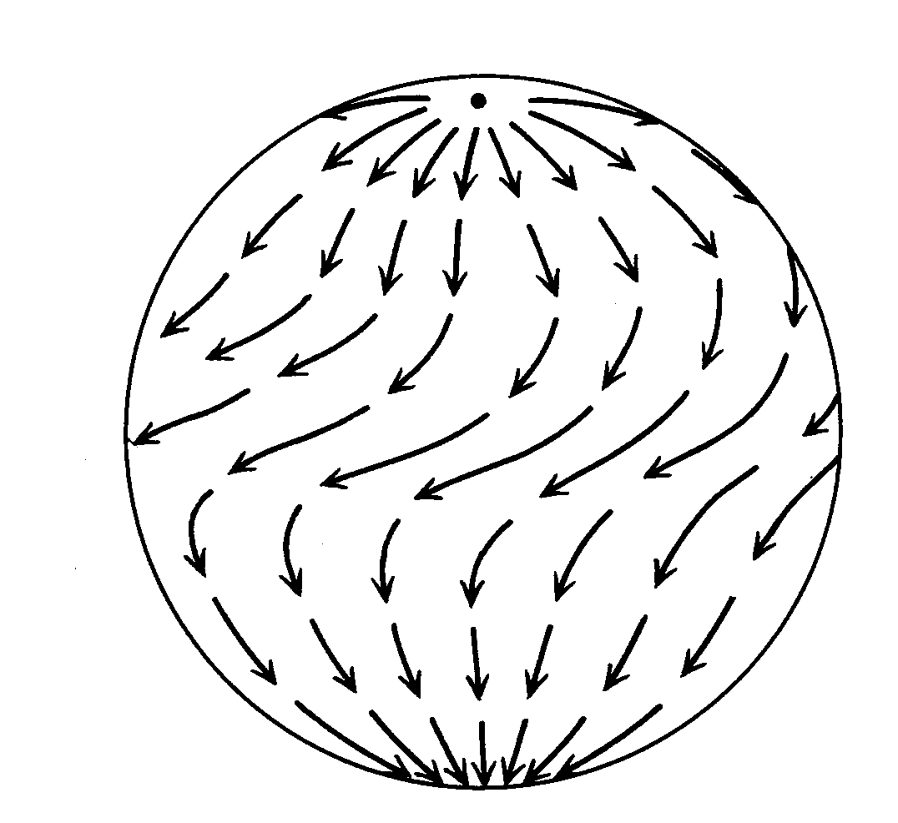
\includegraphics[width=0.33\textwidth]{figures/fig2.4.png}
  \figtitle{2.4}{$X_\theta$（原书 p.64）}
\end{figure}

\begin{figure}[htbp]
  \centering
  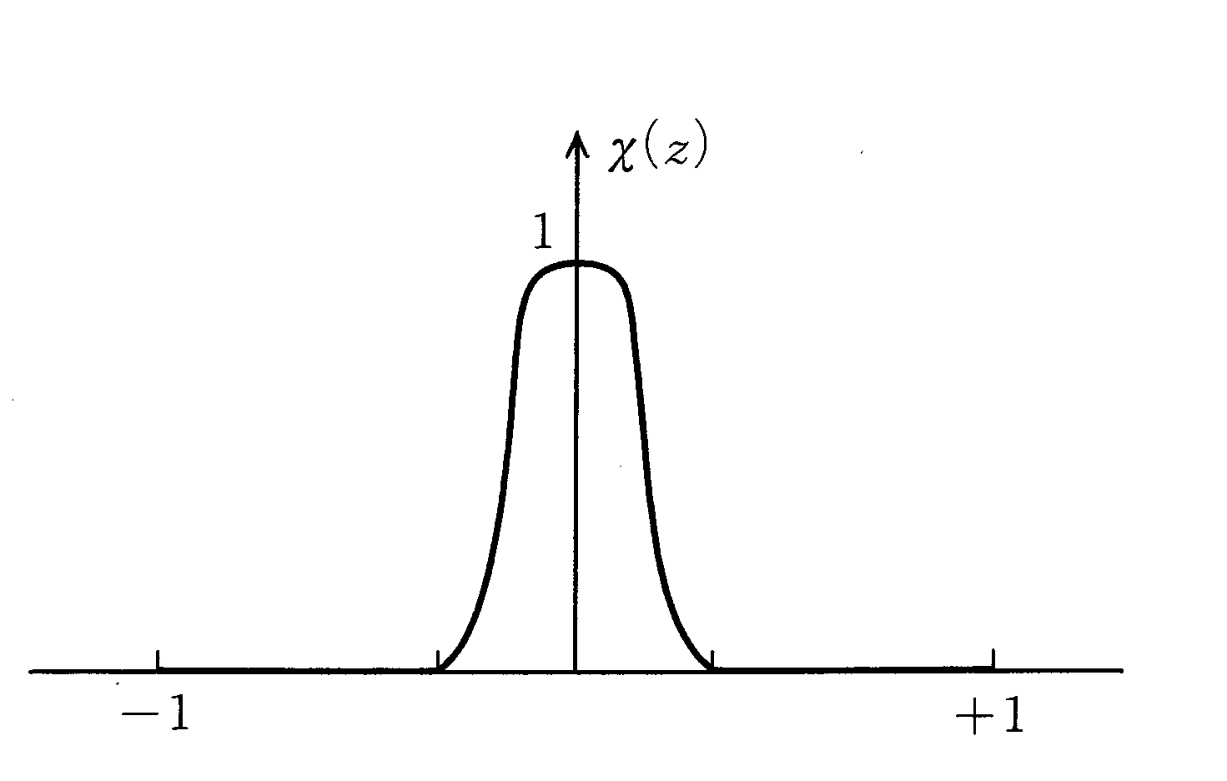
\includegraphics[width=0.46\textwidth]{figures/fig2.5.png}
  \figtitle{2.5}{$\chi(z)$（原书 p.64）}
\end{figure}

然而 $\mathcal{M}_1$ 是空集。因为赤道成为 $X_1$ 的闭轨道，从 $(0,0,1)$ 出发的积分曲线不能越过赤道到达南半球。换一种说法：$\theta$ 接近 $1$ 时，积分曲线越过赤道所需的时间越来越长，$\theta=1$ 时则需要无限长时间。这是因为引理 2.68 在 $\theta=1$ 时不成立。

把 $\theta$ 动起来，画出模空间 $\mathcal{M}=\bigcup_\theta\mathcal{M}_\theta$ 的图形就如图 2.6。请与图 2.1 比较。差别在于 $\mathcal{M}$ 的紧致性。这一点正体现了辛结构的存在与模空间紧致性之间的关系。本节的说明只是这一关系的开端。命题 2.39 的证明还需要更多东西。下文在下一节叙述。

\begin{figure}[htbp]
  \centering
  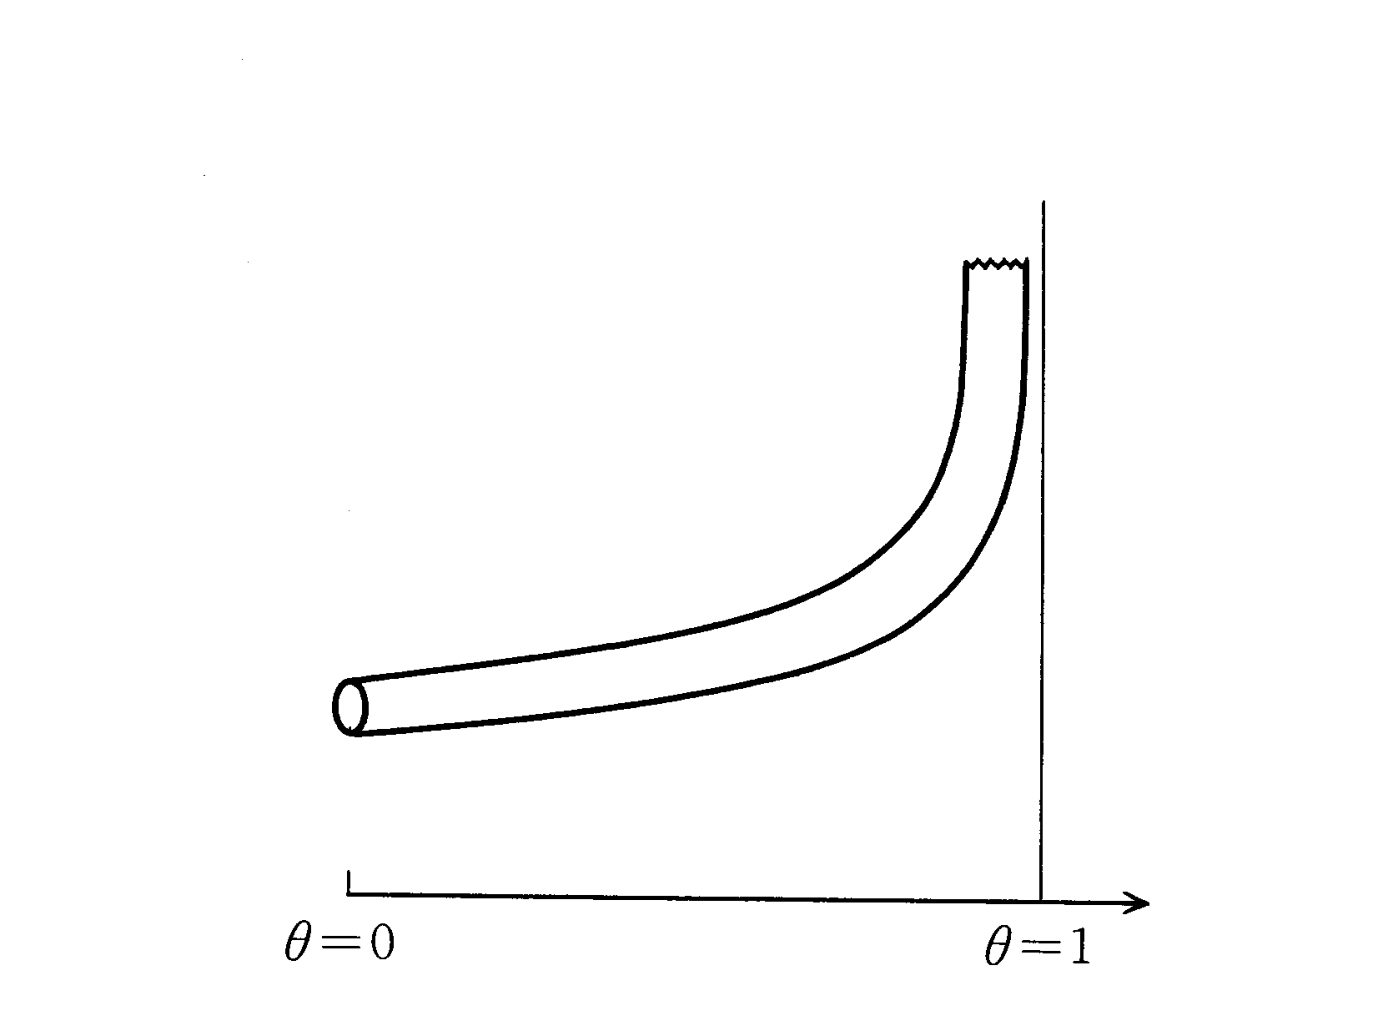
\includegraphics[width=0.52\textwidth]{figures/fig2.6.png}
  \figtitle{2.6}{紧致性崩溃（原书 p.65）}
\end{figure}

% [Tutor Note: $\mathcal{M}_1=\varnothing$ 是“气泡”的有限维模型：$A$ 不再类梯度，引理 2.68 式的能量估计失效，积分曲线在 $\theta\to1$ 时用无穷长时间才越过赤道，模空间的极限点遂从 $S^1$ 上“脱落”。§2.6 的紧化正是要把这种丢失的极限点（气泡）补回来。]

% [原文 p.65]
\section{紧化与气泡}

\takeaway{本节讨论 §2.5 的有限维 Morse 类比在无限维失效的地方：先验估计 $\sup\|d\varphi\|<\infty$（问题 2.88）一般不成立。Sacks–Uhlenbeck 的 $\varepsilon$-正则性给出只依赖能量的局部估计，据此把能量有界的调和映射列的极限写成“光滑映射＋有限个气泡”。}

前一节基于有限维 Morse 理论的类比，讨论了伪全纯映射模空间的紧致性。然而在我们的情形，Morse 函数 $A$ 与有限维的 Morse 函数在许多方面都不相同。本节讨论这些不同之处。本节的内容对比伪全纯曲线更一般的调和映射也成立。

把问题总结一下。设 $\varphi_k\colon\Sigma\to M$ 是从黎曼面 $\Sigma$ 到 $X$ 的伪全纯曲线列。问题在于这一列是否有收敛子列。前一节所说明的是：能量若无界，便不可能收敛。于是假定
\begin{equation}
  \mathcal{E}(\varphi_k)\le C \tag{2.29}
\end{equation}
（定义能量所用的度量取 $\Sigma$ 上的凯勒度量。）按处方 2.87 走一遍吧。(2.29) 可看作那里的 (1)，即关于弱范数的有界性。下一个步骤 (2)（这称为先验的（a priori）估计）就是下面的问题。

\begin{problem}{2.88}
  对满足 (2.29) 的伪全纯映射 $\varphi$，$\sup\|d\varphi\|$ 是否一致有界？
\end{problem}

% [Tutor Note: 原书 p.65 此处作“从黎曼面 $\Sigma$ 到 $X$ 的伪正則曲线列”，据上下文 $X$ 应为 $M$；后文一律用 $M$。]

在前一节的情形，即有限维的 Morse 理论或常微分方程的情形，问题 2.88 总是成立的。也就是说，紧空间上常微分方程解的 $C^1$ 范数总有界。然而在我们的情形，即两个变量的偏微分方程或环路空间上的 Morse 理论，问题 2.88 并不成立。这一困难的发现与克服，是 Uhlenbeck 等人 1970 年代在非线性偏微分方程的几何学研究上的重大成果。先举反例。

% [原文 p.66]
\begin{example}{2.89}
  用 $\varphi_k(z)=z(z+k)/(z+1)$ 定义 $\varphi_k\colon\C P^1\to\C P^1$。由于 $\varphi_k$ 与 $z\mapsto z^2$ 同伦，$\mathcal{E}(\varphi_k)$ 与 $k$ 无关，特别是有界的。然而 $\|d\varphi_k\|$ 在 $0$ 处的值发散。

  即使作定义域 $\C P^1$ 的坐标变换，也不能使 $\|d\varphi_k\|$ 有界。事实上，为使 $0$ 处有界而令 $w=kz$，则 $\varphi_k(w)=w(k^2+w)/(k^2+kw)$。在 $w=\infty$ 附近考虑它。取定义域的（与 $k$ 无关的）坐标变换 $y=1/w$ 与值域的（与 $k$ 无关的）坐标变换 $\psi_k=1/\varphi_k$，得 $\psi_k(y)=y(k^2+ky)/(1+k^2y)$。$\psi_k$ 在 $y=0$（即 $w=\infty$）处的微分发散。
\end{example}

% [Tutor Note: 例 2.89 中 $\psi_k$ 的式子：由 $w=1/y$、$\psi_k(y)=1/\varphi_k(1/y)$ 直接计算应为 $\psi_k(y)=y(k^2y+k)/(1+k^2y)$，原书 p.66 印作 $y(k^2+ky)/(1+k^2y)$，第二项漏了一个因子 $y$，疑为排印之误。结论（$y=0$ 处微分发散）不受影响。]

这种现像称为\textbf{气泡}（bubble）。下面说明气泡为何发生。下面的定理出自 Eells–Sampson [86]，是调和映射理论的出发点。

\begin{theorem}{2.90}
  设 $M$ 是非正截面曲率的紧黎曼流形，$N$ 是任意紧黎曼流形。则对任意映射 $N\to M$，存在与它同伦的调和映射。
\end{theorem}

\begin{remark}{2.91}
  定理 2.90 对 $N$ 的维数不是 $2$ 时也成立。为使读者看出维数为 $2$ 这一假定在何处变得重要，暂时把 $N$ 的维数取为一般。
\end{remark}

回想定理 2.90 证明的要点（详见 [285]）。定理的证明有使用热流（heat flow）的，有直接用变分法的，形形色色，这一点在其他变分问题中也一样。定理 2.90 的证明的特征体现在先验估计上。先验估计不仅用于定理 2.90 这样的存在定理，对本章的主题——模空间的紧化问题——也很重要。因此，就定理 2.90 的情形来证明先验估计。

% [原文 p.67]
先验估计用一句话概括就是：只要 $M$ 具有非正曲率，处方 2.87 的 (2) 就行得通。证明要用下面的 Weitzenböck 公式（Weitzenböck formula）。

\begin{proposition}{2.92}
  设 $N,M$ 如定理 2.90，$\varphi\colon N\to M$ 是调和映射。令 $e_\varphi=\frac12\operatorname{Tr}(\varphi)$。此时
  \[
  \begin{aligned}
    \Delta_Ne_\varphi={}&|\nabla\nabla\varphi|^2
    +\sum_{i,j}g_M\big(d\varphi(\operatorname{Ric}^N(e_i,e_j)e_j),d\varphi(e_i)\big)\\
    &-\sum_{i,j}g_M\big(R^M(d\varphi(e_i),d\varphi(e_j))d\varphi(e_j),d\varphi(e_i)\big)
  \end{aligned}
  \]
  成立。这里 $e_i$ 是 $TN$ 的正交规范基。$\operatorname{Ric}^N$ 是 $N$ 的 Ricci 曲率（Ricci curvature），$R^M$ 是 $M$ 的曲率张量。
\end{proposition}

公式的详细形状并不需要，但要注意下面几点。用 $e_\varphi=\frac12\sum_ig_M(d\varphi(e_i),d\varphi(e_i))$ 把命题 2.92 简写，可表为
\begin{equation}
  \Delta_N(|d\varphi|^2)=|\nabla\nabla\varphi|^2+K_{1,N}|d\varphi|^2-K_{2,M}|d\varphi|^4 . \tag{2.30}
\end{equation}
$K_{1,N}|d\varphi|^2$ 是稍有含糊的记号，大致意思是：它是 $d\varphi$ 的大小的二次式，系数由 $N$ 的曲率决定。$K_{2,M}|d\varphi|^4$ 也类似。

\begin{remark}{2.93}
   Laplace 算子（Laplacian）$\Delta_N$ 的符号有两种流派，这里取 $\Delta_{\R^n}=-\sum_i\dfrac{\partial^2}{\partial x_i^2}$ 这一流派。
\end{remark}

% [Tutor Note: 注意 2.93 的符号约定很要紧：取 $\Delta=-\sum\partial_i^2$ 时，$\Delta_N e_\varphi$ 为“正”算子，故 (2.30) 中 $|\nabla\nabla\varphi|^2$ 的系数是 $+1$，$M$ 非正曲率给出 $-K_{2,M}|d\varphi|^4\ge0$。若换成相反的流仪，则 (2.30) 与引理 2.94 的 $\Delta$ 全要变号。]

看 (2.30) 会发现，几乎所有项关于 $\varphi$ 都是二次的。唯一不是的是最后一项 $K_{2,M}|d\varphi|^4$，它是四次的。(2.30) 各项次数不一，是因为方程（调和映射的方程）是非线性的。换言之，我们所考虑的是非线性方程，这一效应就出现在 $K_{2,M}|d\varphi|^4$ 这一项上。

这里用到 $M$ 具有非正曲率这一假定。于是可知，这一问题的项 $-K_{2,M}|d\varphi|^4$ 总是非负的。因此可以同时舍去这一项与第 $1$ 项，得到下面的引理。（这一论证以及下面引理 2.95 的证明，是 Bochner 技巧的一例。）

\begin{lemma}{2.94}
  在定理 2.90 的假定下，$\Delta_Ne_\varphi+Ce_\varphi\ge0$ 成立。
\end{lemma}

这里要用下面的引理。

% [原文 p.68]
\begin{lemma*}{2.95}
  设 $D^n$（$n$ 维圆盘）上的非负函数 $f$ 满足 $\Delta f+Cf\ge0$，则
  \[
    f(0)\le C'\int_{D^n}f\,dx_1\cdots dx_n .
  \]
  这里 $\Delta$ 是 $D^n$ 上关于与欧氏度量充分接近的度量的 Laplace 算子，$C'$ 是只依赖度量与 $C$ 的常数。
\end{lemma*}

\begin{proof}
  以下用 $\operatorname{dist}$ 表示黎曼流形（这里即 $D^n$）的距离函数。令 $D^n(r)=\{x\in D^n\mid\operatorname{dist}(0,x)\le r\}$，以其边界为球面 $S^{n-1}(r)$。（由于度量与欧氏度量充分接近，$D^n(r)$ 是具光滑边界的 $n-1$ 维球体。）设 $\vec n$ 是 $S^{n-1}(r)$ 的外向法向量。再令 $g(x)=\exp(A\operatorname{dist}(0,x)^2)$（$A$ 是待定的正常数）。用 Green 公式
  \[
    \int_{D^n(r)}(g\Delta f-f\Delta g)\,dx_1\cdots dx_n
    =\int_{S^n(r)}(f\vec n(g)-g\vec n(f))\,\Omega_{S^{n-1}(r)} .
  \]
  由于 $\Delta g<-cA^2g$，只要把 $A$ 取得比只依赖 $C$ 与 $c$ 的某个数大，就有
  \[
    g\Delta f-f\Delta g\ge(\Delta f+cA^2f)g\ge(\Delta f+Cf)g\ge0
  \]
  成立。因此
  \[
    \int_{S^{n-1}(r)}g\vec n(f)\,\Omega_{S^{n-1}(r)}
    \le\int_{S^{n-1}(r)}f\vec n(g)\,\Omega_{S^{n-1}(r)} .
  \]
  于是存在只依赖 $A$ 的 $C_1,C_2$，使
  \[
  \begin{aligned}
    C_1\int_{S^{n-1}(r)}\vec n(f)\,\Omega_{S^{n-1}(r)}
    &\le\int_{S^{n-1}(r)}g\vec n(f)\,\Omega_{S^{n-1}(r)}\\
    &\le\int_{S^{n-1}(r)}f\vec n(g)\,\Omega_{S^{n-1}(r)}
    \le C_2\int_{S^{n-1}(r)}f\,\Omega_{S^{n-1}(r)} .
  \end{aligned}
  \]
  于是令 $h(r)=\int_{S^{n-1}(r)}f\,\Omega_{S^{n-1}(r)}$，则 $dh/dr\le C_2h(r)/C_1$。因此 $h(0)\le\exp(C_2r/C_1)h(r)$ 成立。乘以 $r^{n-1}$ 并从 $0$ 到 $1$ 积分，即得引理。
\end{proof}

% [Tutor Note: 证明中 Green 公式右端的积分区域原书 p.68 印作 $S^n(r)$，按上下文（等式左端是 $D^n(r)$ 的边界）应为 $S^{n-1}(r)$；后面的式子也都用 $S^{n-1}(r)$。此处照抄原书，请读者按 $S^{n-1}(r)$ 读。]

用引理 2.94 可知 $f=e_\varphi$ 满足引理 2.95 的假定。至于“度量与欧氏度量充分接近”这一假定，

% [原文 p.69]
只要乘上常数、放大空间便可满足。于是得到下面的命题。

\begin{proposition}{2.96}
  在定理 2.90 的假定下 $e_\varphi(0)\le C\mathcal{E}(\varphi)$。
\end{proposition}

由命题 2.96 可知，对伪全纯映射 $\varphi$，只要 $M$ 具有非正曲率，就有
\begin{equation}
  |\varphi|_{C^1}\le C\sqrt{\mathcal{E}(\varphi)} \tag{2.31}
\end{equation}
(2.31) 就是先验估计式。

% [Tutor Note: (2.31) 是“$C^1$ 界由能量控制”的显式形式；正因为右端出现 $\sqrt{\mathcal{E}}$，一旦 $M$ 有正曲率、$K_{2,M}|d\varphi|^4$ 不能丢弃，这个估计立刻失效，例 2.89 就是反例。]

那么，现在把 $M$ 的曲率非负这一假定去掉看看。于是 (2.30) 的最后一项不能舍去，上面的证明随之崩溃。

下面要叙述的 Sacks–Uhlenbeck [320] 的定理说的是：只要 $\varphi$ 的能量小，就能回避这一问题。为简单起见，就 $N$ 是 $2$ 维圆盘 $D^2$ 的情形来叙述。（$N$ 不是圆盘时也能作同样的定义，但 $2$ 维这一假定是本质的。）

\begin{theorem}{2.97}
  存在只依赖 $M$ 的正数 $\varepsilon(M),C(M)$，使下述成立。若 $\varphi\colon D^2\to M$ 是调和映射且 $\mathcal{E}(\varphi)\le\varepsilon(M)$，则
  \[
    e_\varphi(0)<C(M)\sqrt{\mathcal{E}(\varphi)} .
  \]
\end{theorem}

例 2.89 表明假定 $\mathcal{E}(\varphi)\le\varepsilon(M)$ 不能去掉。

\begin{proof}
  先证明下面的引理。
\end{proof}

\begin{lemma*}{2.98}
  对任意正数 $A$，存在只依赖 $A$ 与 $M$ 的正数 $C(A,M)$，使下述成立。若 $\varphi\colon D^2\to M$ 是调和映射且 $e_\varphi\le A$，则 $e_\varphi(0)<C(A,M)\mathcal{E}(\varphi)$。
\end{lemma*}

\begin{proof}
  由假定 $e_\varphi\le A$ 与 Weitzenböck 公式 (2.30)，对 $f=e_\varphi$ 可知 $\Delta f+C(1+A)f\ge0$。于是由引理 2.95 即得引理 2.98。
\end{proof}

引理 2.98 的形状与要证的定理 2.97 十分相似，但假定 $e_\varphi\le A$ 等于假定了要证的结论，即关于 $C^1$ 范数的有界性；用它来证定理 2.97，初看像是循环论证。引理 2.98 没有用到那个重要假定——$N$ 是 $2$ 维。下面的两个引理是证明的关键，是 Uhlenbeck 们巧妙避开循环论证的地方。

\begin{lemma*}{2.99}
  设 $x\in D^2$，且 $\operatorname{dist}(x,\partial D^2)>r$。作如下假定。
  \begin{enumerate}[label=（\arabic*）,leftmargin=2.4em]
    \item 对满足 $\operatorname{dist}(x,y)<r$ 的任意 $y$，有 $e_\varphi(y)\le4e_\varphi(x)$。
    % [原文 p.70]
    \item $e_\varphi(x)\le r^{-2}$。
  \end{enumerate}
  此时下面的估计成立。
  \begin{equation}
    e_\varphi(x)<C(2,M)r^{-2}\mathcal{E}(\varphi). \tag{2.32}
  \end{equation}
\end{lemma*}

\begin{proof}
  令 $\varphi'(z)=\varphi(rz+x)$。由 (1),(2) 得 $|\varphi'|_{C^1}\le2$。另一方面，'由于是 $2$ 维'，能量在共形变换下不变（命题 2.73）。因此
  \[
    \mathcal{E}(\varphi')=\int_{\{y\mid\operatorname{dist}(x,y)<r\}}e_\varphi\le\mathcal{E}(\varphi).
  \]
  于是由引理 2.98 即得引理 2.99。
\end{proof}

\begin{lemma*}{2.100}
  存在只依赖 $M$ 的正数 $\varepsilon(M),B(M)$，使下述成立。若 $\varphi\colon D^2\to M$ 是调和映射且 $\mathcal{E}(\varphi)\le\varepsilon(M)$，则对任意 $x\in D^2(1/2)$，$e_\varphi(x)\le100$ 成立。
\end{lemma*}

\begin{proof}
  设引理 2.100 不成立，即
  \begin{equation}
    e_\varphi(x)>100 \tag{2.33}
  \end{equation}
  成立。令 $x_1=x$，$r_1=\sqrt{1/e_\varphi(x_1)}$。另外把 $\varepsilon(M)$ 选得使
  \begin{equation}
    C(2,M)\varepsilon(M)<1 \tag{2.34}
  \end{equation}
  成立。现在对这 $r=r_1$ 考虑引理 2.99。于是由 (2.34) 知结论式 (2.32) 不成立，故必有某个假定不成立。假定 (2) 由 $r_1$ 的取法已经成立。因此下面二者之一成立。
  \begin{enumerate}[leftmargin=3.8em]
    \item[（a1）] $\operatorname{dist}(x_1,\partial D^2)\le r_1$，
    \item[（b1）] $\operatorname{dist}(x_1,x_2)<r_1$，且存在 $x_2$ 使 $e_\varphi(x_2)>4e_\varphi(x_1)$。
  \end{enumerate}
  假定 (b1) 成立。此时令 $r_2=\sqrt{1/e_\varphi(x_2)}$，重复同样的论证。于是
  \begin{enumerate}[leftmargin=3.8em]
    \item[（a2）] $\operatorname{dist}(x_2,\partial D^2)\le r_2$，
    \item[（b2）] $\operatorname{dist}(x_2,x_3)<r_2$，且存在 $x_3$ 使 $e_\varphi(x_3)>4e_\varphi(x_2)$。
  \end{enumerate}
  二者之一成立。如此反复，令 $r_k=\sqrt{1/e_\varphi(x_k)}$，则
  \begin{enumerate}[leftmargin=3.8em]
    \item[（ak）] $\operatorname{dist}(x_k,\partial D^2)\le r_k$，
    \item[（bk）] $\operatorname{dist}(x_k,x_{k+1})<r_k$，且存在 $x_{k+1}$ 使 $e_\varphi(x_{k+1})>4e_\varphi(x_k)$。
  \end{enumerate}

% [原文 p.71]
  二者之一成立。这一过程可以持续到 (ak) 被满足为止。然而
  \[
  \begin{aligned}
    \operatorname{dist}(x_1,x_k)&\le\sum_{j=1}^{k-1}r_j
    \le\sum_{j=1}^{k-1}\sqrt{1/e_\varphi(x_j)}\\
    &\le\sum_{j=1}^{k-1}\sqrt{1/e_\varphi(x_1)}\,2^{-j+1}
    \le2\sqrt{1/e_\varphi(x_1)}\le2\sqrt{1/100}
  \end{aligned}
  \]
  因此 $\operatorname{dist}(x_1,x_k)\le1/4$，故 (ak) 不会成立。也就是说，可以依次选出 $x_k$。

  于是由 $\operatorname{dist}(x_1,x_k)\le1/4$ 与 $\operatorname{dist}(0,x_1)<1/2$，$x_k$ 有收敛到 $D^2$ 内点的子列 $x_{k_i}$。然而 $\lim_{i\to\infty}e_\varphi(x_{k_i})\to\infty$，这与 $e_\varphi$ 连续矛盾。
\end{proof}

\begin{proof}[定理 2.97 的证明（续）]
  定理 2.97 可由引理 2.100 与 2.98 直接得到。
\end{proof}

下面用定理 2.97 证明关于伪全纯映射模空间的下述定理。这是 Uhlenbeck 的定理。

\begin{theorem*}{2.101}
  设 $\varphi_i\colon\Sigma\to M$ 是调和映射的列，且假定 $\mathcal{E}(\varphi_i)\le C$。此时存在子列 $\varphi_{i_\ell}$ 与有限个点 $p_1,\dots,p_J\in\Sigma$，使 $\varphi_{i_\ell}$ 在 $\Sigma-\{p_1,\dots,p_J\}$ 的任意紧集上一致收敛。
\end{theorem*}

\begin{proof}
  对自然数 $k$，按如下方式取 $p_{k,1},\dots,p_{k,N_k}\in\Sigma$。
  \begin{enumerate}[label=（\arabic*）,leftmargin=2.4em]
    \item $\bigcup_jD^2(p_{k,j},1/k)=\Sigma$。这里 $D^2(p_{k,j},1/k)$ 是以 $p_{k,j}$ 为中心、半径 $1/k$ 的球。
    \item $\operatorname{dist}(p_{k,j},p_{k,j'})>1/2k$。
  \end{enumerate}
  这样的 $p_{k,j}$ 可以取到，其证明留给读者。（在满足 (2) 的集合中取极大的 $\{p_{k,1},\dots,p_{k,N_k}\}$，它就满足 (1)。）
\end{proof}

\begin{lemma*}{2.102}
  与 $D^2(p_{k,j_0},2/k)$ 相交的 $D^2(p_{k,j},2/k)$ 的个数不超过 $1000$。
\end{lemma*}

\begin{proof}
  若 $D^2(p_{k,j_0},2/k)\cap D^2(p_{k,j},2/k)\ne\varnothing$，则 $\operatorname{dist}(p_{k,j_0},p_{k,j})\le4/k$。因此
  \begin{equation}
    D^2(p_{k,j},1/4k)\subset D^2(p_{k,j_0},5/k). \tag{2.35}
  \end{equation}
  另一方面由 (2) 得
  % [原文 p.72]
  \begin{equation}
    D^2(p_{k,j},1/4k)\cap D^2(p_{k,j'},1/4k)=\varnothing . \tag{2.36}
  \end{equation}
  $D^2(p_{k,j_0},5/k)$ 的体积（$k$ 大时）约为 $D^2(p_{k,j'},1/4k)$ 的体积的 $20^2=400$ 倍，故由 (2.35),(2.36) 知引理 2.102 成立。
\end{proof}

\begin{proof}[定理 2.101 的证明（续）]
  由引理 2.102，
\[
  \sum_j\int_{D^2(p_{k,j},1/4k)}e_{\varphi_i}\le1000\,\mathcal{E}(\varphi_i)\le1000\,C
\]
成立。因此，使
\begin{equation}
  \int_{D^2(p_{k,j},5/k)}e_{\varphi_i}\ge\varepsilon(M) \tag{2.37}
\end{equation}
成立的 $j$ 的个数，与 $k,i$ 无关地被 $1000C/\varepsilon(M)$ 从上方估计。取子列，设这个数与 $k,i$ 无关，记作 $J$。重排编号，可设使 (2.37) 成立的 $p_{k,j}$ 就是 $p_{k,1},\dots,p_{k,J}$。换言之，设
\begin{equation}
  j>J\ \Longrightarrow\ \int_{D^2(p_{k,j},2/k)}e_{\varphi_i}\le\varepsilon(M) \tag{2.38}
\end{equation}
取子列，可设 $\lim_{\ell\to\infty}p_{k_\ell,j}$ 对任意 $j\le J$ 都收敛。（并设 $\lim_{\ell\to\infty}k_\ell=\infty$ 也成立。）记 $\lim_{\ell\to\infty}p_{k_\ell,j}=p_j$。设 $K$ 是 $\Sigma-\{p_1,\dots,p_J\}$ 的任意紧集。由 (1)，对充分大的 $\ell$ 有
\[
  K\subset\bigcup_{j>J}D^2(p_{k_\ell,j},1/k_\ell)
\]
成立。固定这样一个 $\ell$。注意 $\ell$ 不依赖 $i$，只由 $K$ 决定。取 $z\in D^2(p_{k_\ell,j},1/k_\ell)$。把 $D^2(z,1/k_\ell)$ 的度量放大 $k_\ell$ 倍，在其上应用定理 2.97。由 (2.38)、$D^2(z,1/k_\ell)\subset D^2(p_{k_\ell,j},1/k_\ell)$ 与共形不变性，关于能量的假定是满足的。因此
\[
  e_{\varphi_i}<k_\ell^2C(M)
\]
成立。也就是说，在 $K$ 上 $\varphi_i$ 的 $C^1$ 范数一致有界。于是由 Ascoli–Alzerà 定理，$\varphi_i$ 在 $K$ 上有子列一致收敛。至此证明了：对任意 $K$，$\varphi_i$ 都有子列在 $K$ 上一致收敛。

% [Tutor Note: 定理 2.101 只断言“在去掉有限个点后一致收敛”，并未说明那有限个点附近发生了什么；出问题的那几点正是气泡出现的场所，模空间紧化要额外记录这些点处的“泡泡树”。]

% [原文 p.73]
把“对任意 $K$，$\varphi_i$ 有子列在 $K$ 上一致收敛”翻成“$\varphi_i$ 有子列在任意 $K$ 上一致收敛”，用的是简单的对角线论证。定理 2.101 至此证完。
\end{proof}

% [Tutor Note: 原书 p.72 作“Ascoli–Alzerà 定理”，通名是 Ascoli–Arzelà 定理（紧度量空间上等度连续且有界的函数列有收敛子列），此处照抄原书。]

一句话概括，定理 2.101 是说：能量有界的调和映射列，除有限个点外收敛。发散的点可能存在，例 2.89 正说明了这一点。

\begin{remark}{2.103}
  定理 2.101 只讲了一致收敛。其实调和映射总是光滑的，而且一旦一致收敛，连各阶导数也一起一致收敛。这一事实是椭圆型方程的一般理论，这里不予证明。参见 [141] 等。
\end{remark}

\begin{remark}{2.104}
  定理 2.101 中没有变动 $M$ 及其上的度量。当 $M$ 上有一列度量 $g_{M,k}$、而 $\varphi_k\colon\Sigma\to(M,g_{M,k})$ 是调和映射时，只要列 $g_{M,k}$ 的极限存在且仍是 $M$ 的度量，用完全相同的证明便得到完全相同的结论。
\end{remark}

属于先验估计的还有另一个非常重要的定理，称为可去奇点定理（removable singularity theorem）。

\begin{theorem}{2.105}
  设 $\varphi\colon D^2-\{0\}\to M$ 是调和映射，且
  \[
    \int_{D^2-\{0\}}e_\varphi<\infty .
  \]
  此时 $\varphi$ 可延拓为 $D^2$ 上的光滑映射。
\end{theorem}

定理 2.105 是伪全纯曲线理论的基石。其证明见 [25] Chapter 5、[253] §4.2 等。

以上都是对一般 $M$ 成立的事实。现在回到定理 2.36 的情形，把迄今为止的考察用到命题 2.39 的证明上。设 $\varphi_k\colon S^2\to\C P^2$ 是 $\mathcal{M}_{\tau_k}$ 的元素的列，设 $\lim\tau_k=\tau$。要证明的是 $\lim\varphi_k$ 收敛。由假定的 $\varphi_k[S^2]=[\C P^1]$ 与引理 2.78，能量的有界性随之成立，故由定理 2.101 与注 2.103, 2.104，$\varphi_k$ 在去掉有限个点 $\{p_1,\dots,p_J\}$ 后收敛。把其极限记作 $\varphi$。
\begin{equation}
  \int_{S^2-\{p_1,\dots,p_J\}}e_\varphi
  =\sup_{K\subset S^2-\{p_1,\dots,p_J\}}\int_Ke_\varphi
  =\sup_K\lim_{k\to\infty}\int_Ke_{\varphi_k} \tag{2.39}
\end{equation}

% [原文 p.74]
\[
  \le\sup_K\lim_{k\to\infty}\int_{S^2}e_{\varphi_k}
  \le[\C P^1]\cap[\omega_{\C P^2}].
\]
因此可用定理 2.105，$\varphi$ 延拓为 $S^2$ 上的映射。仍用同一记号表示。其实想证明的是 $\lim\varphi_k=\varphi$。

首先，设 $0,1,\infty$ 中至少有两点在 $\{p_1,\dots,p_J\}$ 之外。于是可知 $\varphi$ 不是常值映射。（例如，若 $1$ 与 $\infty$ 不在 $\{p_1,\dots,p_J\}$ 中，则在该处 $\lim\varphi_k=\varphi$，故由假定 $\varphi(1)=[1:0:1]\ne[1:1:0]=\varphi(\infty)$。）因此 $\int_{S^2}e_\varphi\ne0$。另一方面 $\int_{S^2}e_\varphi=\varphi_*([S^2])\cap\omega_{\C P^2}$。因此
\begin{equation}
  \int_{S^2}e_\varphi\ge[\C P^1]\cap[\omega_{\C P^2}]. \tag{2.40}
\end{equation}
（$[\C P^1]$ 曾是 $H^2(\C P^2,\Z)$ 的生成元。）也就是说，(2.39) 中等号成立。

由此，对 $j=1,\dots,J$ 存在 $c_j$，使
\[
  \int_{D^2(p_j,c_j)}e_{\varphi_k}<\varepsilon(\C P^2)
\]
对充分大的任意 $k$ 成立。于是放大 $1/\sqrt{c_j}$ 倍后用定理 2.97，便知在 $p_j$ 的邻域内 $\varphi_k$ 的 $C^1$ 范数也一致有界。也就是说，$\varphi_k$ 在整个 $S^2$ 上收敛。

最后，假定 $\varphi_k$ 在 $3$ 点 $0,1,\infty$ 中的 $2$ 点以上发散，导出矛盾。设它在 $0,1$ 处发散。取 $0$ 的邻域 $D^2(0,r)$，使 $D^2(0,2r)\cap\{p_1,\dots,p_J\}=\{0\}$。取 $z_k\in D^2(0,r)$ 使
\begin{equation}
  e_{\varphi_k}(z_k)=\sup_{z\in D^2(0,r)}e_{\varphi_k}(z). \tag{2.41}
\end{equation}
由于 $e_{\varphi_k}$ 在 $0$ 处发散、在 $D^2(0,r)$ 的边界上收敛，$z_k$ 存在且 $\lim z_k=0$。令 $r_k^2=e_{\varphi_k}(z_k)^{-1}$，定义 $\phi_k(z)=\varphi_{z_k+z/r_k}$。$\phi_k$ 是 $D^2(0,r_k)\to M$ 的映射。由 (2.41)，$\phi_k$ 的 $C^1$ 范数不超过 $1$。因此 $\phi_k$ 在 $\C=S^2-\{\infty\}\to M$ 的映射意义下紧一致收敛。设极限为 $\phi$，则可知 $\phi$ 的能量有限，故 $\phi$ 可延拓为 $S^2\to M$ 的映射（定理 2.105）。

% [原文 p.75]
于是与 (2.40) 同样可得
\[
  \int_{S^2}e_\phi\ge[\C P^1]\cap[\omega_{\C P^2}]
\]
由此，对充分大的 $k$ 有
\[
  \int_{D^2(0,r)}e_{\varphi_k}>(1-\delta)[\C P^1]\cap[\omega_{\C P^2}].
\]
对 $1$ 的邻域作同样的考察，得
\[
  \int_{D^2(1,r)}e_{\varphi_k}>(1-\delta)[\C P^1]\cap[\omega_{\C P^2}].
\]
取 $r$ 足够小，可使 $D^2(0,r)\cap D^2(1,r)=\varnothing$。于是
\[
  \int_{S^2}e_\varphi>2(1-\delta)[\C P^1]\cap[\omega_{\C P^2}].
\]
这与 (2.39) 矛盾。


% [Tutor Note: 这一步正是“气泡”的正式表述：$\phi_k(z)=\varphi_{z_k+z/r_k}$ 把 $0$ 附近按 $1/r_k\to\infty$ 的倍率放大，得到的极限 $\phi$ 是把气泡（一张 $S^2$）吹到极限映射上；$\phi$ 的能量恰为 $[\C P^1]\cap[\omega]$，故 (2.40) 与 (2.39) 中的上界对撞而产生矛盾。]

以上省略了不少细节，也没有证明定理 2.105，但定理 2.36 已几乎证明完毕。

\begin{remark}{2.106}
  最近 Taubes [359] 用 monopole 方程与 Seiberg–Witten 不变量把定理 2.36 作了如下推广。对 $\C P^2$ 上任意辛结构 $\omega$ 与关于 $\omega$ 温和的近复结构，存在伪全纯映射 $S^2\to\C P^2$，其同调类为 $[\C P^1]$ 或 $-[\C P^1]$。作为应用（用 Gromov 在 [159] 中的结果），可以证明 $\C P^2$ 上的辛结构在相差常数倍的意义下唯一。

  这一结果在辛拓扑与 $4$ 维拓扑两方面都受到关注，是与 $4$ 维辛流形分类问题相关的重要结果。这方面可看 [224], [230] 等。Taubes 还用伪全纯曲线与 monopole 方程研究 $4$ 维退化辛结构，正在得到有趣的结果（[360], [361]）。

  Donaldson 关于辛子流形存在性的结果 [77], [78]（适用范围比 $4$ 维更广）也是这方面的重要结果。
\end{remark}

% [原文 p.76]
\section{最初的应用}

\takeaway{本节用 §2.3–§2.6 的全套工具证明 Gromov 非挤压定理：$R>r$ 时球 $D^{2n}(R)$ 不能辛嵌入 $D^2(r)\times\C^{n-1}$。关键是把问题化到 $S^2(S)\times T^{2n-2}$ 上伪全纯球面的存在性（定理 2.108），再用单调性估计与面积比较得出矛盾。}

\footnote{本节的叙述依据 [25] 的 Introduction。}定理 2.107 称为非挤压定理（non-squeezing theorem），是 Gromov 在 [159] 中证明的、宣告大范围辛几何诞生的定理。$D^{2n}(R)$ 指向量空间 $\C^n$ 中半径为 $R$ 的球。$\C^n$ 上取标准辛结构。

\begin{theorem}{2.107}
  若 $R>r$，则 $D^n(R)$ 与 $D^2(r)\times\C^{n-1}$ 的任何开子集都不辛同胚。
\end{theorem}

% [Tutor Note: 原书 p.76 定理 2.107 及 p.78 引理 2.110 把球体写作 $D^n$，而本节开头把它定义为 $\C^n$ 中半径 $R$ 的球 $D^{2n}(R)$，证明中也一律用 $D^{2n}$。据上下文 $D^n$ 应为 $D^{2n}$ 之误，此处照抄原书。]

由定理 2.107 可知，例如 $D^2(2)\times D^2(1/2)$ 与 $D^2(1)\times D^2(1)$ 不辛同胚。这是问题 2.14 中最早找到的反例。空间 $D^2(2)\times D^2(1/2)$、$D^2(1)\times D^2(1)$ 二者都是简单到不能再简单的空间，然而定理 2.107 的证明要用到 §2.3 至 §2.6 所述的一切，离自明甚远。

定理 2.107 的证明要用下面的定理 2.108，它的证法与定理 2.36 相同。在 $2n$ 维环面 $T^{2n}=\C^n/\Z^n$ 上取由 $\C^n$ 的标准辛结构导出的辛结构 $\omega_{T^{2n}}$。（这样的辛结构并不唯一，取哪个都行。）令 $S^2(S)=\partial D^3(S)$。在 $S^2(S)\times T^{2n-2}$ 上取直积辛结构 $\omega_{S^2(S)\times T^{2n-2}}$。设 $J_{S^2(S)\times T^{2n-2}}$ 是关于 $\omega_{S^2(S)\times T^{2n-2}}$ 温和的任意近复结构（未必可积）。取任意点 $(p_0,q_0)\in S^2(S)\times T^{2n-2}$。

\begin{theorem*}{2.108}
  存在伪全纯曲线 $\varphi\colon S^2\to S^2(S)\times T^{2n-2}$，使 $\varphi(0)=(p_0,q_0)$ 且同调类为 $[S^2\times\mathrm{pt}]$。
\end{theorem*}

\begin{proof}
  与定理 2.36 几乎相同，故简述。取 $\omega_{S^2(S)\times T^{2n-2}}$ 温和的近复结构族 $J_\theta$，使 $J_0$ 为直积复结构、$J_1$ 为 $J_{S^2(S)\times T^{2n-2}}$。取 $q_1,q_2\in S^2(S)$，把满足 $\varphi(0)=(p_0,q_0)$、$\varphi(1)\in\{q_1\}\times T^{2n-2}$、$\varphi(\infty)\in\{q_2\}\times T^{2n-2}$ 的关于近复结构 $J_\theta$ 的伪全纯曲线 $\varphi$ 中同调类为 $[S^2\times\mathrm{pt}]$ 的全体记作 $\mathcal{M}_\theta$。把 $\mathcal{M}_\theta$ 在 $\theta\in[0,1]$ 上的并集

  % [原文 p.77]
  记作 $\mathcal{M}$。容易看出 $\mathcal{M}_0$ 只有一点。又由指数定理（或 Riemann–Roch 定理）知 $\mathcal{M}_\theta$ 的虚拟维数为 $0$。因此只要 $\mathcal{M}$ 紧，便可与定理 2.36 的证明同样地证明 $\mathcal{M}_1$ 非空，即定理 2.108。紧致性也照定理 2.36 的情形同样证明。最后一步（相当于 §2.6 最后的论证的部分）要用到 $\pi_2(S^2(S)\times T^{2n-2})\cong\Z$ 且 $[S^2\times\mathrm{pt}]$ 是其生成元。
\end{proof}

\begin{proof}[定理 2.107 的证明]
  设 $R>r$，导出矛盾。取满足 $R>R'>r'>r$ 的 $R',r'$。考虑与 $D^2(r')$ 面积相等的球面 $S^2(S)=S^2(r'/2)$。设 $D\subset S^2(S)$ 是与 $D^2(r)$ 面积相等的圆盘（小圆围成的图形），则 $D^2(r)$ 与 $D$ 辛同胚。（证明留给读者。）把这个辛同胚记作 $\bar\Psi$。由 $\bar\Psi$ 导出 $\Psi\colon D^2(r)\times T^{2n-2}\to S^2(S)\times T^{2n-2}$。

  设 $\tilde F\colon D^{2n}(R)\to D^2(r)\times\C^{n-1}$ 是到像上的辛同胚。取充分大的 $C$，可设 $\tilde F$ 导出嵌入 $\bar F\colon D^{2n}(R)\to D^2(r)\times\C^{n-1}/C\Z^{2n-2}$。这里 $\C^{n-1}/C\Z^{2n-2}=T^{2n-2}$。$\bar F$ 与 $\Psi$ 的合成给出嵌入 $F\colon D^{2n}(R)\to S^2(S)\times T^{2n-2}$。把 $D^{2n}(R)$ 上的标准复结构用 $F$ 搬过去，得到 $F$ 的像上的、与 $\omega_{S^2(S)\times T^{2n-2}}$ 相容的近复结构。把这个近复结构在 $F(D^{2n}(R'))$ 之外稍作改动，便可延拓为 $S^2(S)\times T^{2n-2}$ 上的、与 $\omega_{S^2(S)\times T^{2n-2}}$ 相容的近复结构 $J_{S^2(S)\times T^{2n-2}}$。（可用引理 2.26 证明。）

  令 $(p_0,q_0)=F(0)$，对 $J_{S^2(S)\times T^{2n-2}}$ 应用定理 2.108。把所得的 $\varphi(S^2)$ 用 $F$ 拉回。设 $\Sigma$ 是 $F^{-1}(\varphi(S^2))$ 中含 $0$ 的连通分支。由 $\varphi(0)=F(0)$ 知 $\Sigma$ 非空。又因 $\varphi$ 的同调类不为 $0$，它也不是常值映射。
\end{proof}

% [Tutor Note: 原书 p.77 此处作“对 $J_{S^2(S)\times T^{2n-2}}$ 应用定理 2.107”，据上下文应为定理 2.108（存在伪全纯球面）；定理 2.107 正是本节要证的目标，不可能在此被引用。此处照抄原书。]

\begin{lemma*}{2.109}
  $[\Sigma]\cap\omega\le\pi r'^2$。
\end{lemma*}

\begin{proof}
  由于 $F$ 是辛同胚，
  \[
    [\Sigma]\cap\omega=\int_{F(\Sigma)}\omega_{S^2(S)\times T^{2n-2}} .
  \]

  % [原文 p.78]
  由于 $\varphi$ 是伪全纯映射，$\varphi^*(\omega_{S^2(S)\times T^{2n-2}})$ 在任意开集上的积分为正。因此
  \[
    \int_{F(\Sigma)}\omega_{S^2(S)\times T^{2n-2}}
    \le\int_{S^2}\varphi^*(\omega_{S^2(S)\times T^{2n-2}})=\pi r'^2 .
  \]
\end{proof}

由下面的引理，定理 2.107 的证明即告完成。

\begin{lemma*}{2.110}
  $\Sigma$ 的面积不小于 $\pi R'^2$。
\end{lemma*}

\begin{proof}
  设 $D^n(t)$ 是以原点为中心、半径为 $t$ 的球。令 $L(t)=\partial D(t)\cap\Sigma$，$A(t)=D(t)\cap\Sigma$。$L(t)$ 是 $1$ 维的，$A(t)$ 是 $2$ 维的。用 $\ell(t)$ 表示 $L(t)$ 的长度，用 $a(t)$ 表示 $A(t)$ 的面积。
  \begin{equation}
    \frac{da(t)}{dt}\ge\ell(t) \tag{2.42}
  \end{equation}
  成立。考虑 $L(t)$ 的锥 $CL(t)=\{sx\mid s\in[0,1],\ x\in L\}$，则 $CL(t)$ 的面积为 $t\ell(t)/2$。因此，由于 $\Sigma$ 面积最小，
  \begin{equation}
    a(t)\le\frac{t\ell(t)}{2} \tag{2.43}
  \end{equation}
  由 (2.42),(2.43) 得
  \[
    \frac{d}{dt}\frac{a(t)}{t^2}=\frac{t\dfrac{da(t)}{dt}-2a(t)}{t^3}\ge0 .
  \]
  在 $0$ 附近放大，$\Sigma$ 越来越接近平面，故 $\lim_{t\to0}a(t)/t^2=\pi$。因此 $a(t)\ge\pi t^2$。取 $t=R'$ 即得引理。
\end{proof}

\begin{remark}{2.111}
  引理 2.110 可推广到非欧氏度量的情形，称为单调性原理（monotonicity principle）。也有用单调性原理证明定理 2.97 或 2.105 的流派（见 [298], [299], [404]）。
\end{remark}

% [Tutor Note: 引理 2.110 的证明里 $D^n(t)$、$\partial D(t)$ 沿用了原书 $D^n$ 的写法，应按 $D^{2n}(t)$、$\partial D^{2n}(t)$ 读（$D^{2n}$ 是 $\C^n$ 中的球）。关键一步是 $t\mapsto a(t)/t^2$ 单调不减，故其最小值只能在 $t\to0$ 处取得，而 $t\to0$ 时 $\Sigma$ 趋于平面、比值趋于 $\pi$；这正是“单调性”一词的由来。]

\begin{remark}{2.112}
  这里给出的定理 2.107 的证明中，考虑不可积的近复结构起了核心作用。定理 2.107 不是复几何的定理，而是辛几何的定理。例如在镜像对称中伪全纯曲线的应用里，这一点就更为含糊。
\end{remark}

% [原文 p.79]
下面给出定理 2.107 的一个重要应用。它属于 Eliashberg [91]\footnote{以下的证明本质上归功于 Gromov。Eliashberg 的证明与此不同。}。

\begin{theorem}{2.113}
  设 $\varphi_k\colon(M,\omega_M)\to(M,\omega_M)$ 是辛同胚，且 $\lim_{k\to\infty}\varphi_k$ 按 $C^0$ 收敛于微分同胚 $\varphi\colon M\to M$。此时 $\varphi$ 是辛同胚。
\end{theorem}

\begin{remark}{2.114}
  若不按 $C^0$ 收敛而按 $C^1$ 收敛，定理的结论是显然的。
\end{remark}

定理 2.113 也称为辛拓扑的存在定理等。倘若辛同胚群在所有微分同胚群中 $C^0$ 稠密，大范围辛几何便不可能有值得一看的内容。这就是这个名称的由来。

% [Tutor Note: 注意 2.114 与定理 2.113 合起来说的是：辛同胚群在 $C^1$ 拓扑下显然是闭的（保持 $\omega$ 是闭条件），而在 $C^0$ 拓扑下也闭，则是 Gromov 刚性这一非平凡事实。若只有 $C^1$ 闭性，辛同胚群完全可能被微分同胚群 $C^0$ 逼近而不等于其闭包。]

\begin{lemma*}{2.115}
  设 $A\in SL(2n;\R)$，并假定 $A,-A\notin Sp(n;\R)$。则存在 $\R^{2n}$ 的基 $e_i,f_i$ 与 $B\in Sp(n;\R)$，满足下述性质。
  \begin{enumerate}[label=（\arabic*）,leftmargin=2.4em]
    \item $\omega(e_i,e_j)=\omega(f_i,f_j)=0$，$\omega(e_i,f_j)=\delta_{ij}$。这里 $\omega$ 是 $\R^{2n}$ 的辛形式，$\delta_{ij}$ 是 Kronecker 的 $\delta$。
    \item 存在 $0<\lambda<1$，使 $B(A(e_1))-\lambda e_1$、$B(A(f_1))-\lambda f_1$ 含于 $e_2,\dots,e_n,f_2,\dots,f_n$ 张成的线性子空间。
    \item 对 $i\ge2$，$B(A(e_i)),B(A(f_i))$ 含于 $e_2,\dots,e_n,f_2,\dots,f_n$ 张成的线性子空间。
  \end{enumerate}
\end{lemma*}

\begin{proof}
  存在 $e,f$ 使 $|\omega(e,f)|\ne|\omega(Ae,Af)|$。由 $A\in SL(2n;\R)$，可设 $|\omega(e,f)|=\lambda^2|\omega(Ae,Af)|<|\omega(Ae,Af)|$。存在 $B_1\in Sp(n;\R)$ 使 $B_1A(e)=\lambda e$、$B_1A(f)=\lambda f$。

  把 $e,f$ 张成的向量空间关于辛形式的正交补记作 $\langle e,f\rangle^\perp$。存在 $B_2\in Sp(n;\R)$ 使 $B_2B_1A$ 保持 $\langle e,f\rangle^\perp$。还可设 $B_2$ 满足 $B_2e-e\in\langle e,f\rangle^\perp$、$B_2f-f\in\langle e,f\rangle^\perp$。

  令 $B=B_2B_1$、$e_1=e$、$f_1=f$，并选取 $e_2,\dots,e_n,f_2,\dots,f_n$ 使之成为 $\langle e,f\rangle^\perp$ 的基，则引理的结论得到满足。
\end{proof}

\begin{proof}[定理 2.113 的证明]
  这是局部问题，故可在 $\R^{2n}$ 中考虑。$\varphi_k$ 保持
  % [原文 p.80]
  $\R^{2n}$ 的 Lebesgue 测度。因此其 $C^0$ 极限也保持 Lebesgue 测度。也就是说，$\varphi$ 的微分属于 $SL(2n;\R)$。也容易看出 $\varphi$ 保持定向。因此，若 $\varphi$ 不是辛同胚，则由引理 2.115，通过合成（线性）辛同胚，可设 $d_0\varphi$ 具有引理 2.115 中 $BA$ 应满足的性质。即
  \[
    f(x_1,y_1,\dots)=(\lambda x_1,\lambda y_1,\dots)
  \]
  在忽略 $2$ 次以上项的意义下成立。因此，取充分小的 $\varepsilon$ 与满足 $\varepsilon>\varepsilon'>\lambda\varepsilon$ 的 $\varepsilon'$，便有 $f(D^{2n}(\varepsilon))\subset D^2(\varepsilon')\times\C^{n-1}$。这与定理 2.107 矛盾。
\end{proof}

本节所述诸结果由 Hofer 等人作了很大发展。它与本书未能充分叙述的、辛几何中动力系统研究的潮流相关。关于伪全纯曲线对动力系统的应用，[182] 是基本文献。另见 [17], [31], [89] 等。最近还听到定理 2.107 的无穷维推广及其应用（[228], [51]）。

\chapterreview{%
本章是全书的技术枢纽。第 1 章的历史叙述在此落成一套可操作的工具：近复结构、伪全纯曲线、模空间、紧致性；此后第 3 至第 6 章的几乎每个论断，都要回到本章的语言才能读懂。换个说法，本书后面证明的定理，大半是本章方法的变奏。

脉络可以这样串起来。§2.1 给出定义与例，§2.2 用 Darboux 与 Moser 两定理说明辛几何在局部没有不变量，正是这一“局部贫乏”把兴趣逼向整体。§2.3 引入近复结构与 Hermite 度量，使辛流形上出现复几何式的方程，并把“与 $\omega$ 相容”弱化为“关于 $\omega$ 温和”，为后来的扰动论证留出余地。§2.4 搭起 Fredholm 框架，把模空间当作 Fredholm 映射的原像，用 Sard–Smale 型定理与隐函数定理得到正则值的横截性。§2.5、§2.6 处理紧致性：先借 Morse 理论作有限维类比，指出 $A$ 不过是环路空间上的多值函数，再把“$C^1$ 界由能量控制”这一先验估计与 Sacks–Uhlenbeck 的局部 $\varepsilon$-正则性拼起来，得到除有限个点外收敛。§2.7 以非挤压定理收束全章。

核心结论有两条。其一是命题 2.39：伪全纯曲线的模空间在加入气泡后紧。其二是定理 2.107：辛球不能挤压进细长的柱体。二者靠同一件事相连——能量有界的伪全纯曲线只能以气泡的方式失去紧性，而真正阻止气泡出现的，是辛结构而非近复结构。§2.7 末尾的定理 2.113 把这一点推向极端：辛同胚的 $C^0$ 极限仍是辛同胚，故辛同胚群在微分同胚群中并不 $C^0$ 稠密。

需要辨析的有三处。其一，定理 2.97 的局部估计只在能量足够小时成立，全局紧致性必须靠紧化补上气泡，两者不可混为一谈；书中“能量有界则收敛”一类说法都要这样读。其二，本章交替使用“与 $\omega_M$ 相容”与“关于 $\omega_M$ 温和”两个假设：前者还要求 $J$ 保持辛形式，后者只保证 $g_M$ 正定；命题 2.62 用前者，引理 2.85 用后者，读者须随时确认用的是哪一个。其三，$A$ 只在覆盖空间 $\widetilde\Omega_0(M)$ 上单值，式 (2.21) 中的常数 $c(\gamma)$ 是后来 Floer 同调取 Novikov 环系数的伏笔。

作者的写法以类比先行、技术押后，好处是动机清楚、几何图像鲜明，代价是 Fredholm 理论、Sobolev 估计与指数定理被压缩成黑箱；正文多处“留给读者”“省略”正落在这里。与第 3 章动量映射的 Morse 理论、第 5 章 Floer 同调衔接时，这些黑箱需读者自行补齐，这也是本章宜与 [25]、[253] 对读的原因。全章未引入一般性的 Gromov–Witten 不变量，把计数问题留到第 6 章，这一安排在成书的 1999 年是恰当的，今天读来则略感铺垫偏长。%
}

% CHUNK ch02b DONE

